\documentclass{beamer}

\usepackage{tikz}
\setbeamertemplate{navigation symbols}{}

\usepackage{xfp}
\ExplSyntaxOn
\let\intmodnn\int_mod:nn
\ExplSyntaxOff

\begin{document}
	
\foreach \x in {11.25,11.20,...,-12}{	
	\begin{frame}[plain]
		\begin{tikzpicture}[remember picture, overlay]
			\node at (current page.center) {
\includegraphics[width=\paperwidth]{Phantom_Background}};
			\ifnum \intmodnn{\thepage}{6} > 2
			 	\node[yshift=-1cm] at (current page.center) {
\includegraphics[width=\paperwidth]{Phantom_Candels}};
			\else
				\node[yshift=-1cm] at (current page.center) {
\includegraphics[width=\paperwidth]{Phantom_Candels2}};
			\fi
			\node[xshift=\x cm,yshift=-1cm] at (current page.center) {
\includegraphics[width=\paperwidth]{Phantom_Ship_Top}};
			\node[xshift=\x cm,yshift=-1cm] at (current page.center) {
\includegraphics[width=\paperwidth]{Phantom_Erik}};
			\node[xshift=\x cm,yshift=-1cm] at (current page.center) {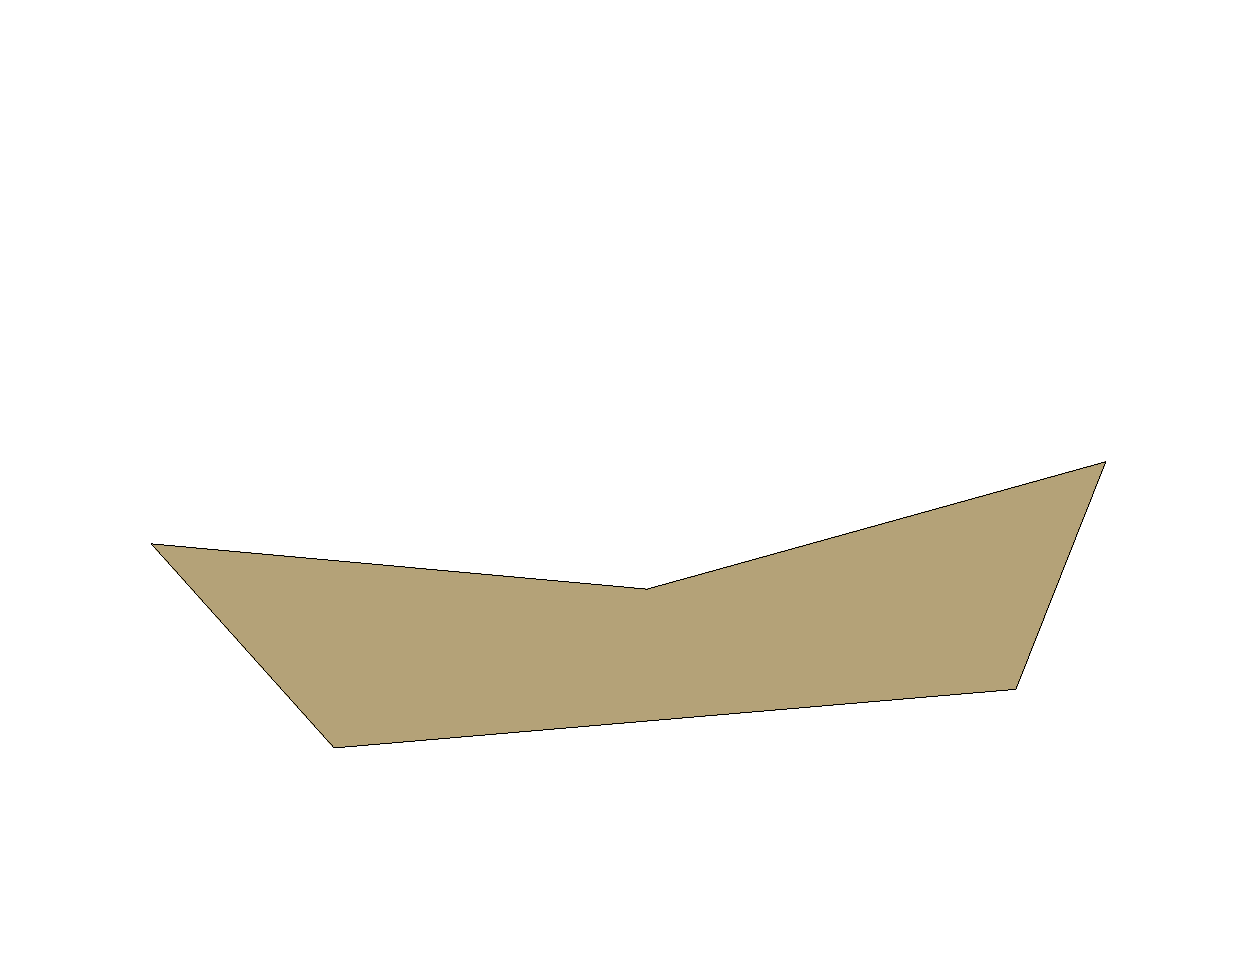
\includegraphics[width=\paperwidth]{Phantom_Ship_Bottom}};
			\node[xshift=\x cm,yshift=-1cm] at (current page.center) {
\includegraphics[width=\paperwidth]{Phantom_Christine}};
		\end{tikzpicture}	
	\end{frame}	
}
	
\end{document}